\documentclass[]{interact}

\usepackage{amsmath}
\usepackage{graphicx}
\usepackage[caption=false]{subfig}
\usepackage{siunitx}
\usepackage{cleveref}
\usepackage{booktabs}
\usepackage{multirow}
\usepackage[natbibapa,nodoi]{apacite}

% \usepackage{soul}
% \DeclareRobustCommand{\tofix}[1]{{\sethlcolor{yellow}\hl{[#1]}}}
\usepackage{color}
\newcommand{\tofix}[1]{\textcolor{red}{\bf{[#1]}}}

\setlength\bibhang{12pt}
\renewcommand\bibliographytypesize{\fontsize{10}{12}\selectfont}

\begin{document}

\articletype{Review Draft}

\title{Experimental Analysis of a Spatialised Audio Interface for People with Visual Impairments}

\author{%
  \name{Jacobus C. Lock\textsuperscript{a}\thanks{Contact Author}, Iain D. Gilchirst\textsuperscript{b}, Grzegorz Cielniak\textsuperscript{a} and Nicola Bellotto\textsuperscript{a}}%
  \affil{\textsuperscript{a}University of Lincoln, Lincoln, LN6 7TS, UK; \textsuperscript{b}University of Bristol, Bristol, BS8 1TH, UK}%
}

\maketitle

\begin{abstract}
  Sound perception is a fundamental skill for many people with severe sight impairments.
  The research presented in this paper is part of the ActiVis project, the aim of which is to build a mobile guidance aid to help people with limited vision find objects in an unknown environment.
  This system requires an effective non-visual interface and uses bone-conduction headphones to transmit audio instructions to the user.
  It has been implemented and tested with spatialised audio cues, which convey the direction of a predefined target in 3D space.
  We present an in-depth evaluation of the audio interface with several experiments that involve a large number of participants, both blindfolded and with actual visual impairments, and analyse the pros and cons of our design choices.
  In addition to producing state-of-the-art results, we found that Fitts's Law can be used to form a metric that can be used to improve and refine the quality of the audio interface in future mobile navigation aids. 
\end{abstract}

\begin{keywords}
  Visual impairment; active vision; guidance system; audio interface; Fitts Law
\end{keywords}

\section{Introduction}

The ActiVis\footnote{https://lcas.github.io/ActiVis/} project aims to build an indoor mobile navigation aid for people with vision impairments that can guide them to their destination in the last leg of their journey (the so-called `last 10-yard problem').
Improvements to computer vision and machine learning techniques, as well as mobile commuting hardware improvements are exploited to make this system possible.
In particular, techniques from the active vision field are being used to enable a mobile device to gather information on the surrounding environment and use it to generate guidance instructions for a user with limited or no vision.
However, in literature, these techniques are typically limited to electro-mechanical servos~\citep{bajcsy2018revisiting} and in this project, we attempt to find out if the same techniques can also be used to direct a user's attention to a certain point. 
In previous work we implemented a prototype system that uses active vision and machine learning models to gather information and help a person find objects in an unknown environment, showing that these techniques can indeed successfully be applied to humans as well~\citep{lock2019active}.

The prototype platform is based on a Google Project Tango\footnote{https://en.wikipedia.org/wiki/Tango\_(platform)} device, pictured in \Cref{fig:tango} and \Cref{fig:tango-headphone}, that embeds a colour camera and provides access to powerful real-time localisation (through IMU measurements and landmark tracking) and image-processing facilities. 
It also provides access to Android's full range of interface tools and I/O options. 
Furthermore, a set of bone-conduction headphones (pictured in \Cref{fig:tango-headphone}), which are placed on a user's cheekbones instead of their ears and do not interfere with normal hearing, are used to transmit the audio signals to the user.

\begin{figure}[t]
  \centering
  \subfloat[]{\label{fig:tango}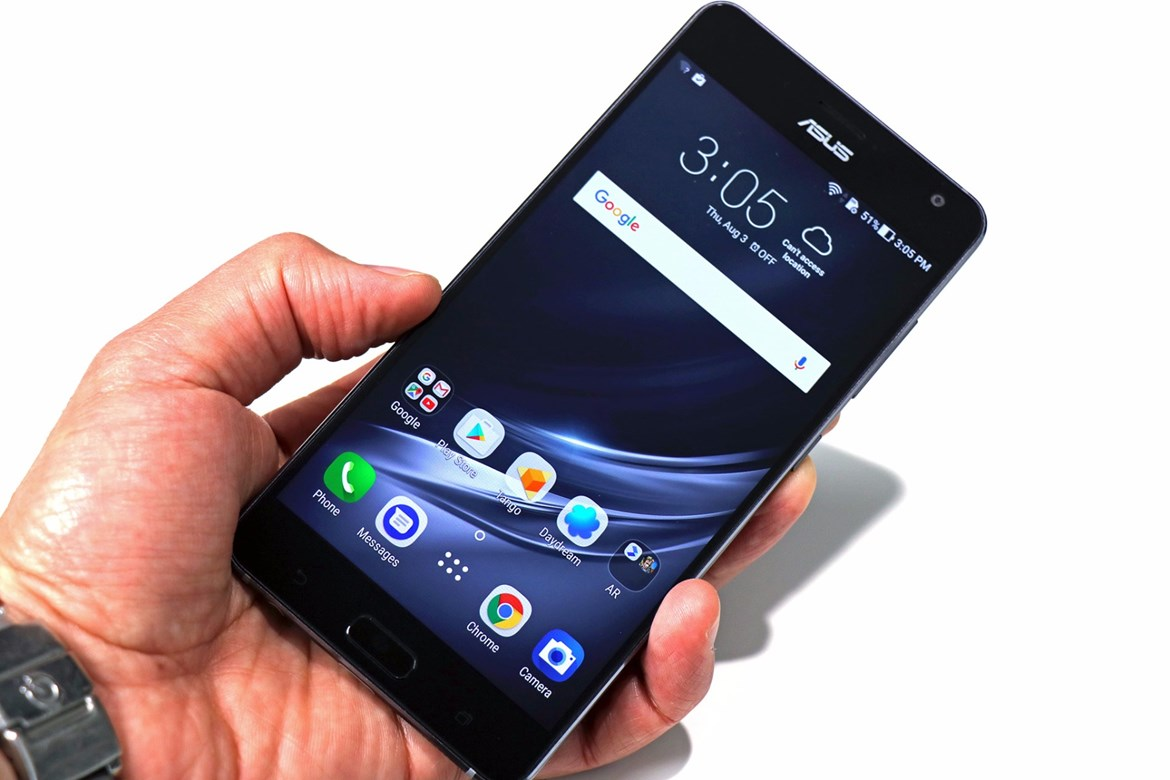
\includegraphics[width=0.4\columnwidth]{figures/tango_asus.jpeg}}
~
  \subfloat[]{\label{fig:tango-headphone}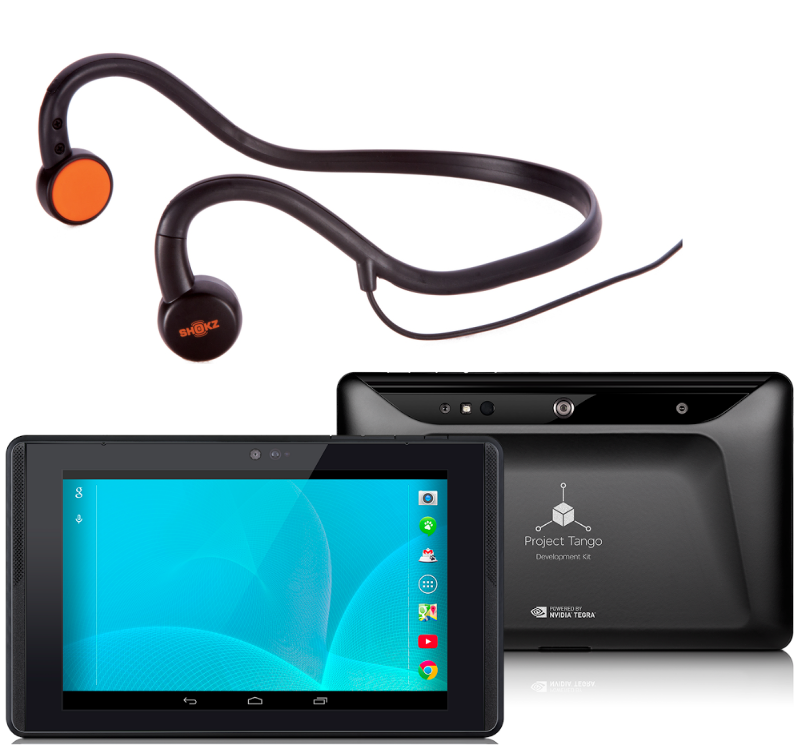
\includegraphics[width=0.3\columnwidth]{figures/tango_headphone.png}}
~
  \subfloat[]{\label{fig:participant}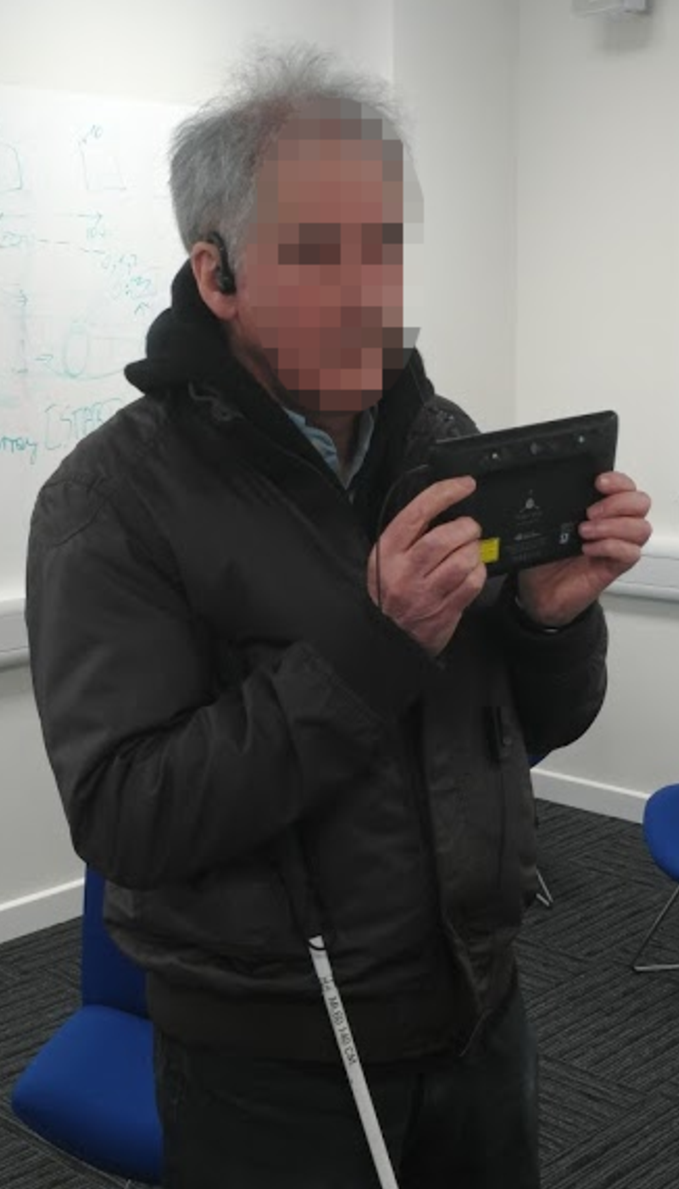
\includegraphics[width=0.2\columnwidth]{figures/vi_participant.pdf}}
  \caption{Pictures of the latest Tango mobile phone (left), the former Tango tablet and the bone-conduction headphones used in this work (centre), and a participant with visual impairments during an experiment (right)~\citep{lock2019bone}.}
\end{figure}

Humans are able to determine the 3D position of a sound source and by exploiting this natural ability, the real-time guidance instructions can be interpreted without posing a significant cognitive load.
A sound source can be spatialised by adjusting a tone's spectral make-up (elevation angle), time delay and level difference (pan angle), and intensity (distance).
In our case, only the pan and elevation positions are transmitted to the user to point the camera towards a target object or visual feature.
However, since bone-conduction headphones bypass the outer ear structure, their spectral signature cannot properly be interpreted and we therefore convey the target's elevation angle by adjusting the tone's pitch.
In previous work, we showed that this audio signal transmission scheme can direct users to a target position with a degree of accuracy comparable to fully spatialised signals sued with expensive closed-cup headphones~\citep{lock2019bone,macdonald2006spatial} and we expand upon this initial investigation with a larger dataset and look at if, and how, changing the behaviour of the pitch affects target acquisition performance in terms of time and angular error. 
The participants' hearing characteristics are also measured to determine if there are limitations to how well they can determine audio pitch or direction. 

The main contributions of this paper are two-fold: 

\begin{itemize}
  \item we provide more comprehensive experimental results on how well a tone with varying pitch can convey a target's tilt angle when using a mobile device with bone-conducting headsets; 
  \item we show that this sound-based human-machine interface conforms to Fitts's Law and can provide a useful metric of performance for similar mobile user interfaces.
\end{itemize}

The rest of the paper starts by discussing previous relevant works and research in \Cref{sec:prev-work}, followed by a discussion on the design and implementation of our interface in \Cref{sec:system-description}.
This is followed by a description of the experiments that were conducted and a discussion of their results in \Cref{sec:experiments} and \Cref{sec:results}.
Finally, the paper concludes with a summary and a short discussion on future research prospects in \Cref{sec:conclusion}.

\section{Previous Work}\label{sec:prev-work}

Multiple mobile navigation and travel aids have been devised throughout the years, some as part of a commercial undertaking and many as part of academic research.
The majority of these systems rely on one or a combination of vocal~\citep{mocanu2016when,chessa2016integrated,kanwal2015navigation}, audio~\citep{schwarze2015intuitive,rodriguez2012obstacle,katz2010navig} and haptic~\citep{rivera-rubio2015assistive,lee2015rgb,xiao2015assistive} feedback media to communicate guidance instructions to the user, each with their own sets of features and limitations.
In general, participants with visual impairments report that they prefer haptic and vocal feedback out of the three options~\citep{arditi2013user}.
However, haptic feedback systems typically have extra hardware requirements to transmit the guidance instructions.
Furthermore, haptic and vocal feedback can become a cognitive burden, particularly where high resolution guidance, which can exceed the bandwidth of these particular senses, is required.
Indeed, participants report that they would prefer control over the vocal feedback channel and trigger guidance instructions, instead of being given constant guidance instructions~\citep{arditi2013user}.
Simple audio tones are less affected by these bandwidth and hardware limitations, but they can potentially fatigue the user's senses if too unpleasant.

Simple audio tones and vocal feedback signals have been used in conjunction with cameras and object detectors to communicate their relative positions to the user with a reasonable level of accuracy~\citep{schauerte2012assistive,tian2013computer,fiannaca2014headlock,vazquez2012helping}.
Following this, researchers have investigated using audio signals that are spatialised with a head-related transfer function (HRTF), simulating a sound source located at some arbitrary 3D position~\citep{geronazzo2016interactive,wilson2007swan,katz2010navig,blum2013spatialized}.
The authors generally report favourable results for this guidance approach when used with standard over-ear headphones or speakers. 
However, other authors have found that the choice of audio transmission medium can have a significant effect on performance.
Cheaper headphones and bone-conduction headphones generally report unfavourable results when compared to over-ear or more expensive alternatives~\citep{schonstein2008comparison,macdonald2006spatial,stanley2006lateralization}. 
This seems to be limited to the elevation dimension, however, and can be improved with HRTFs adjusted for the bone-conduction pathway~\citep{stanley2006lateralization}.
~\cite{durette2008visuo} transmit a target's elevation angle by adjusting the signal's pitch and report favourable results. 
We extended on the latter's work and investigated spatial audio for guidance mode closely in an initial study and found that it is indeed able to adequately guide a user towards a target area~\citep{lock2019bone}.
We expand upon this preliminary study with a more thorough investigation into the participants' performance and how changes to the audio signal's behaviour can impact that performance.

Researchers have previously used Fitts's Law~\citep{fitts1954information}, and more recently MacKenzie's modified version of it~\citep{mackenzie1992fitts}, as a metric to evaluate the performance of a spatial audio HMI\@.
Fitts's Law was originally proposed for visual target search tasks, but has since been applied in non-visual target search tasks as well.
For example, experiments with a haptic feedback pointing device have been performed to evaluate how effective it was at directing a user towards a target~\citep{ahmaniemi2009augmented} and the authors showed that the search time adheres to Fitts's Law.
However, they also note that it is not a perfect fit, citing the fact that Fitts's Law does not take into account a user's search strategy.
Another group of researchers conducted experiments using a spatial audio interface to describe the position of a target on the horizontal plane~\citep{marentakis2006effects}.
Here, participants pointed to where they thought the targets were, on their left or right, as they traversed a path.
Their results show a good relation between target difficulty and search time, providing a strong argument that Fitts's Law can be used to describe the performance of a spatial audio interface.
These results have since been supported by other authors, who found that Fitts's Law provided a good explanation for the results from an experiment using visual, limited visual and non-visual feedback cues~\citep{wu2010fitts}.
However, Fitts's Law has not yet been shown to apply to a spatial tone that uses varying pitch to convey the target's tilt angle, as demonstrated in this paper.

\section{System Description}\label{sec:system-description}

Existing electronic navigation aids have typically struggled to gain market traction and replace the traditional walking cane as the standard assistive tool for people with visual impairments.
Current technological limitations include prohibitive costs, bulky hardware requirements and non-user-friendly interfaces~\citep{golledge2004stated,yusif2016older,arditi2013user}.
To address these issues, we implemented a handheld mobile system that is based on a concept proposed by~\cite{lock2019active} and tested by~\cite{lock2019bone} using a Google Tango device that is able to localise itself in real-time.
This system has the benefit of minimal hardware requirements and a compact, familiar form-factor, which will help to overcome the hurdle of user-acceptance and usability.

A set of bone-conduction headphones is used as the audio transmission medium.
These headphones sit on a user's cheekbones and conduct the audio signals through the skull into the inner ear, instead of through the outer part like typical over-ear headphones. 
This has the benefit of allowing the user access to ambient sounds and noise, so a person with limited vision can still relies on sound to detect, for example, oncoming vehicles and people~\citep{lichtenstein2012headphone}.
Alternative solutions that allow ambient noise through, such as open-back headphones, were also considered, but they still filter the incoming sound and were therefore disregarded.
The AfterShockz headphones (\Cref{fig:tango-headphone}) were ultimately selected since they do not interfere on other sounds and are also more discreet than the larger over-ear headphones. 

\subsection{Audio Interface}

Humans localise a sound source in three dimensions by considering cues recorded in one ear (monaural cues) and comparing cues received at both ears (binaural cues)~\citep{blauert1997spatial,blauert1969sound}.
The binaural cues include inter-aural time and level differences (ITD and ILD respectively) that help to determine a source's location on the horizontal plane.
Monaural cues are taken from the interaction of the sound with the human anatomy, e.g.\ head, shoulders, outer ear, before it enters the ear canal.
When the modified audio signal enters the inner ear canal, the human brain is able to analyse the frequency response and accurately determine the position of the sound source on the median plane. 
The distance to the source is simply derived as the intensity, or volume, of the source, i.e.\ a louder sound would appear closer to the user than a softer one. 

When an audio signal is transmitted via a set of speakers or headphones, it can be transformed with an HRTF to mimic the characteristics of a natural sound source before it is transmitted, making the brain believe a sound is located at some arbitrary position.
An HRTF is a mathematical function that simulates the response signal of a human head and is derived by capturing key characteristics that affect the monaural and binaural responses, such as the user's hearing levels and head size.
Since hearing responses are unique amongst different users, the best results would be observed if each user had their own customised HRTF.\
However, given the complicated process involved to capture the required user characteristics, making unique HRTFs is often an untenable solution and using average values (e.g.\ head measurements, height, etc.) have shown to produce acceptable results~\citep{gardner1995hrtf}.

The guidance information is presented to the user in terms of pan and elevation angles, indicating the angular adjustments required to point the device camera at the target location, as shown in \Cref{fig:cam-coords}.
Spatialised audio signals are well-suited to the task, displaying similar levels of performance to vocal feedback, but with less cognitive load and higher resolution~\citep{klatzky2006cognitive}.
However, given the previously discussed limitations of bone-conduction and spatialised audio, we propose a simple linear adjustment to the signal's pitch as a function of the elevation angle. 
The pan angle, instead, can be conveyed by transforming the audio signal with an HRTF, and indeed it has been found that this dimension is unaffected by using bone-conduction headphones~\citep{schonstein2008comparison,macdonald2006spatial,stanley2006lateralization}. 

\begin{figure}[t]
  \centering
  \subfloat[]{\label{fig:cam-coords}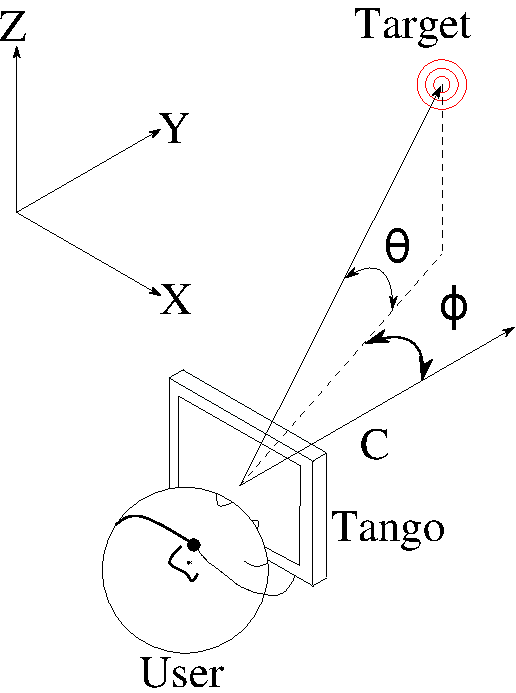
\includegraphics[width=0.3\columnwidth]{figures/camera_coordinate.pdf}}
\hfil
  \subfloat[]{\label{fig:pitch-gain}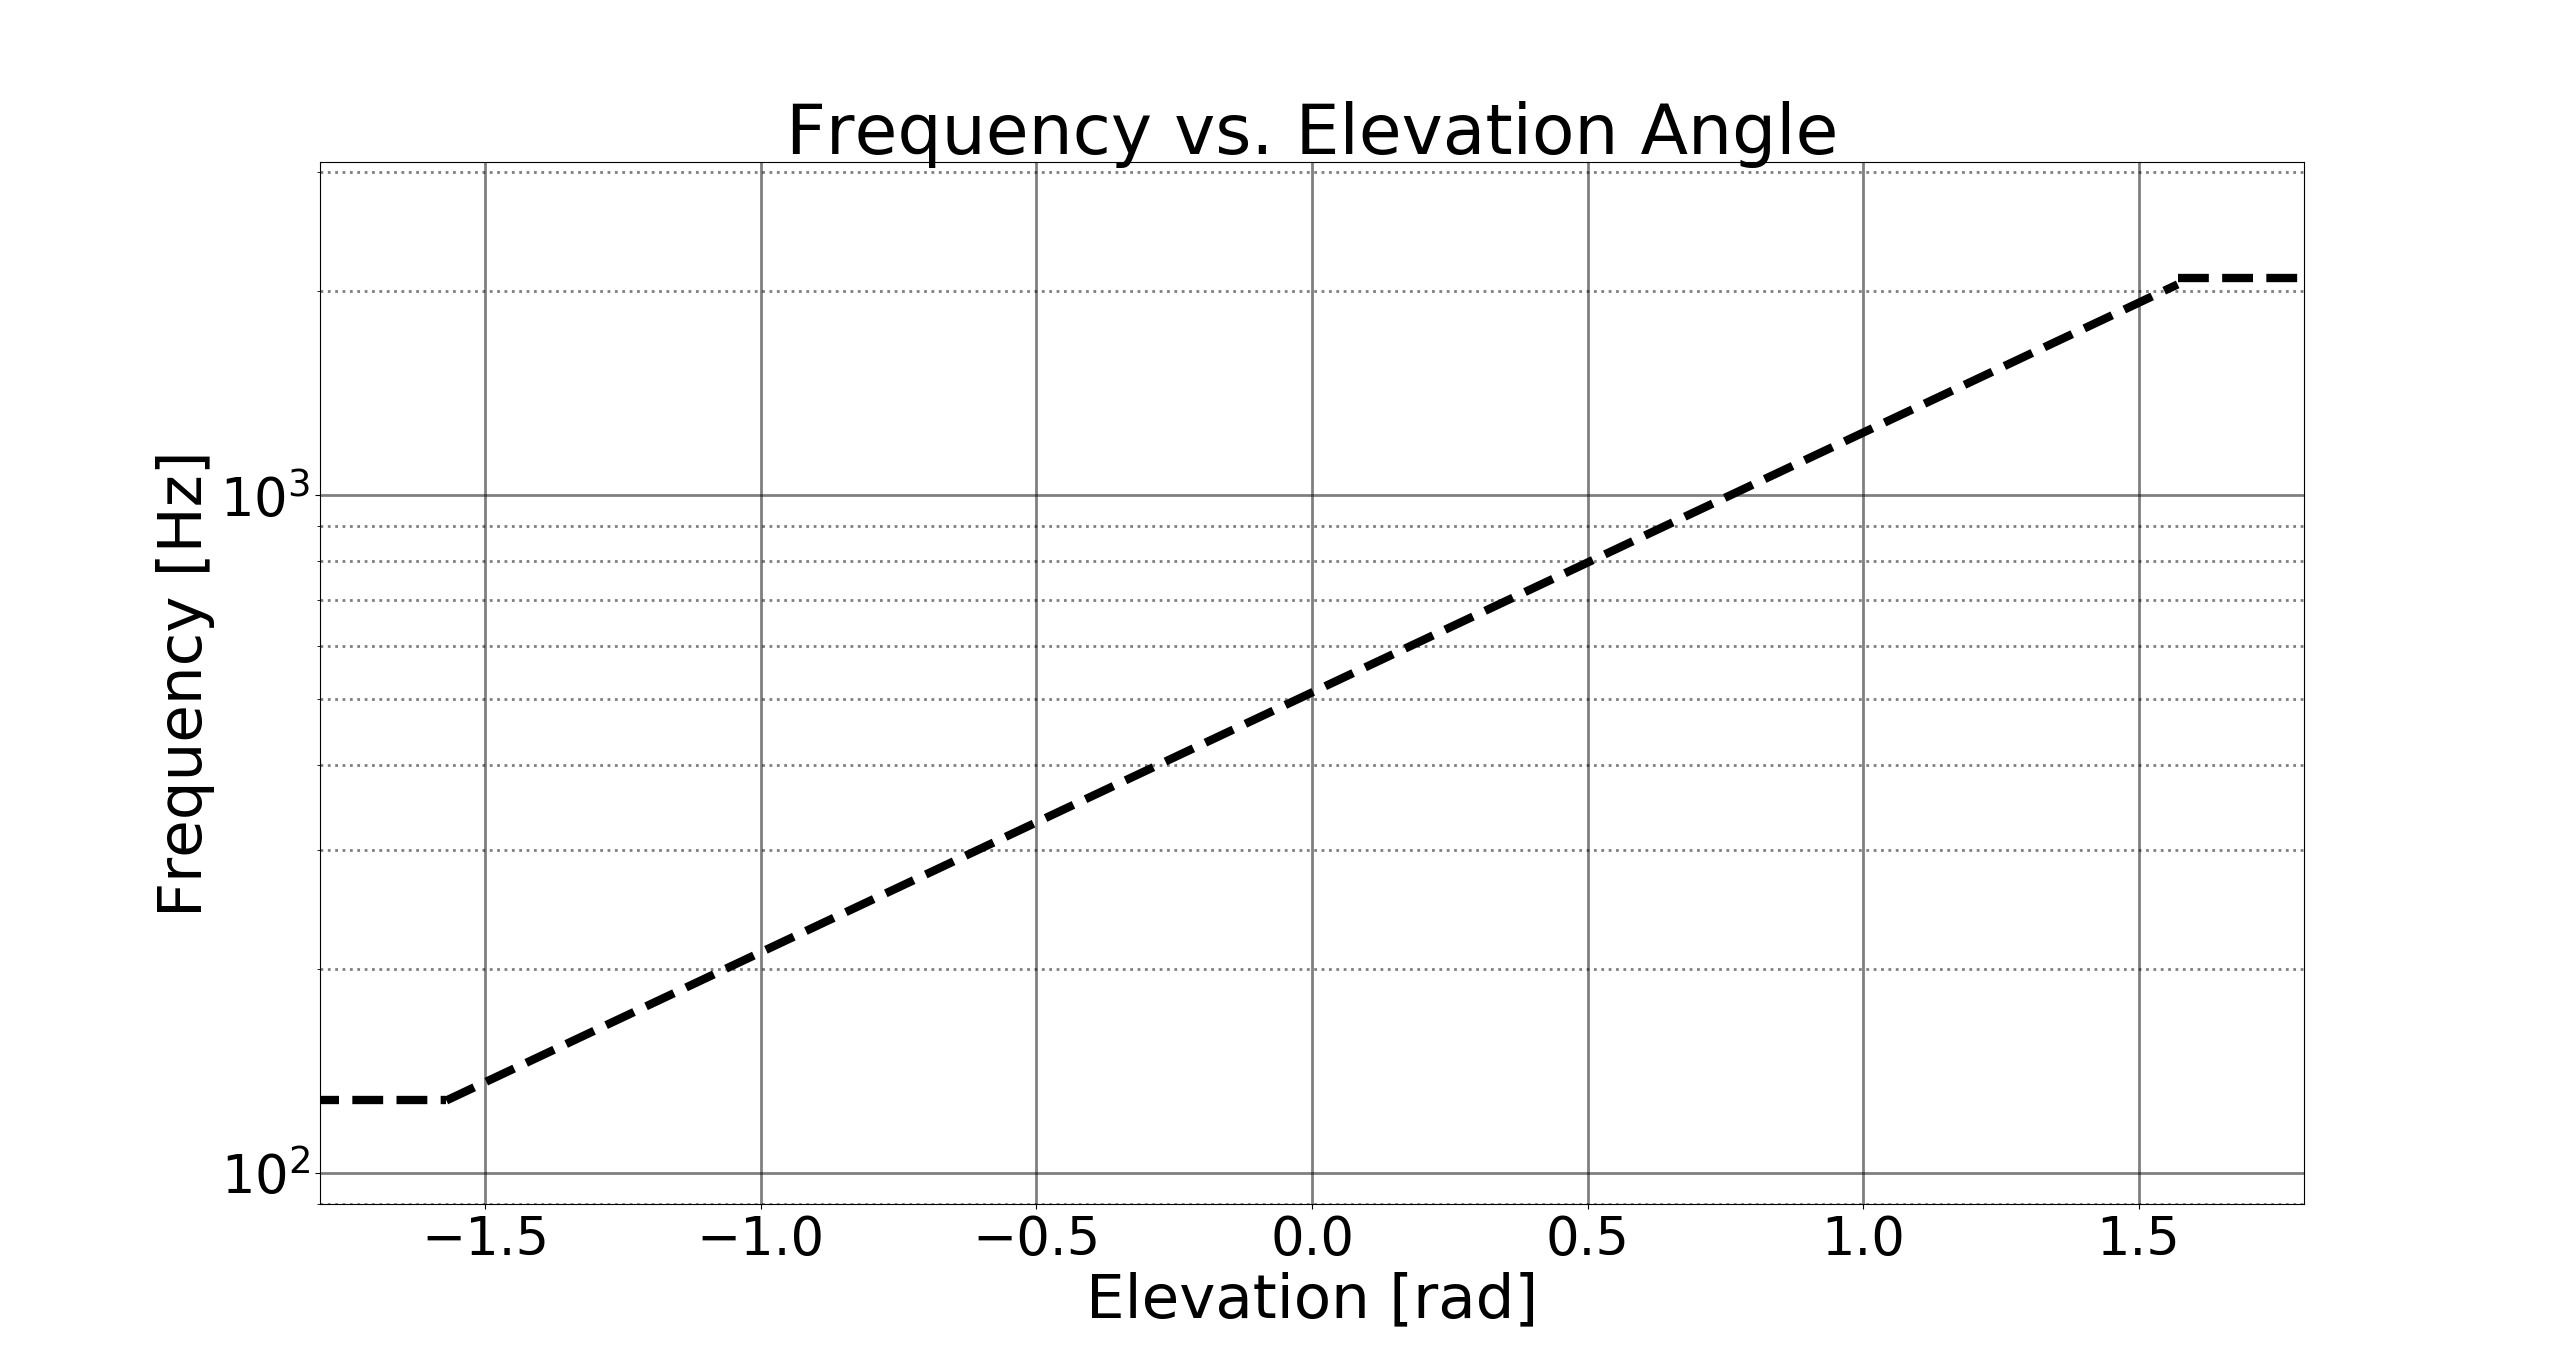
\includegraphics[clip, trim=0 0 0 40, width=0.7\columnwidth]{figures/pitch_gain_function.png}}
  \caption{The reference system used by the guidance interface showing the camera vector and pan and elevation angles (left) and the pitch gain function used to convey the target's elevation angle (right). Note the logarithmic scale of the frequency axis~\citep{lock2019bone}.}
\end{figure}

\subsubsection{Pan Dimension}

The human audition system uses binaural comparison cues, such as ITD and ILD, to localise a sound source on the horizontal plane~\citep{blauert1969sound}.
The ITD is the perceived time delay between the signal reaching both ears, while the ILD is the perceived volume difference in the signal.
For example, a sound that comes from the individual's right will hit the right ear first with a slightly higher volume.

In this work, a pure sinusoidal wave was used. 
People typically have trouble localising a pure tone without a sufficiently rich spectral signature.
However, the ITD and ILD are independent of the tone's spectral make-up, while the elevation angle is given through a different mechanism. Therefore, a pure sine wave is suitable to convey the target's pan angle.
To transform and spatialise the audio signal, we used OpenAL's default HRTF, based on the MIT's KEMAR dataset~\citep{hiebert2005openal}, which uses the person and targets' positions as input, and outputs a transformed audio signal.

\subsubsection{Elevation Dimension}

A generic HRTF implementation with bone-conduction headphones is not very effective in conveying the elevation angle of a sound source~\citep{macdonald2006spatial,schonstein2008comparison}.
To compensate for this, we communicate the target's elevation angle by adjusting the tone's pitch (i.e.\ the sine wave's frequency) as a function of the elevation. 
When the camera vector is at the correct elevation, the tone pitch is set to neutral.
When the target is above or below the camera vector, the pitch is increased or decreased, respectively.
This high/low association scheme is motivated by humans' natural association of high-pitched sounds with elevated sound sources, and low-pitched sounds with source's below the individual's earline~\citep{pratt1930spatial,blauert1997spatial}.
An octave- and semitone-based function is used to adjust the tone's pitch to ensure perceptible changes, while keeping the timbre roughly constant~\citep{shepard1964circularity}.
The pitch is updated at a rate of \SI{10}{\hertz} and changes as the user moves the device.

The pitch is changed as a linear function of the elevation angle and the gradient is determined by setting the angle and pitch limits.
For this work, we only consider a \SI{180}{\degree} field of view in front of the user and limit the elevation angle to a range of \SI{\pm90}{\degree}, or $[-\frac{\pi}{2}, \frac{\pi}{2}]$.
After practical tests with the interface, we set the neutral, on-target pitch the HMI emits to \SI{512}{\hertz}, which is comfortably audible and allows for a large number of suitable octave limits to be selected.
The pitch limits are set at some integer number of octaves above and below the neutral, on-elevation pitch.
After practical tests with the interface, we set the neutral pitch to \SI{512}{\hertz}, which is comfortably audible and allows for a large number of suitable octave limits to be selected.
We set the pitch limits to two octaves away from the neutral pitch, giving frequency limits of [\SI{128}{\hertz}, \SI{2048}{\hertz}].
The linear function is visualised in \Cref{fig:pitch-gain}.

\section{Experiments}\label{sec:experiments}

We performed a set of experiments with the audio interface to determine how effective it is at directing a user to adjust the pan and elevation angles of a camera for point it to a target.
Furthermore, we also carried out a set of pre-screening experiments to determine each participant's hearing characteristics.
The participants were given time before the experiments commenced to familiarise themselves with the device and the tones it emits, as well as what the `on-target' tone sounds like.
We also tested the system with a group of severely sight impaired participants and compared their data to the blindfolded dataset.
The results from the experiments we performed allow us to better understand how the users respond to different settings for the spatial audio feedback stimulus and use them to improve and optimise the behaviour of the feedback modes in our portable navigation aid.

\subsection{System Setup}

A diagram of the experimental system pipeline is shown in~\Cref{fig:pipeline}, where the arrows indicate the direction of the information flow.
When the user taps the Tango's screen, a new virtual target is generated and its coordinates are sent to the audio generation module, along with the device's current position and orientation.
The audio generator then produces a tone based on the difference between the device and the target's positions. The tone is sent to the audio output channel, which plays it back to the user.
A WiFi recording module is constantly monitoring the different values of the device's parameters and of the target's position, as well as the system's output, recording everything in a remotely stored datafile. 

\begin{figure}[t]
  \centering
  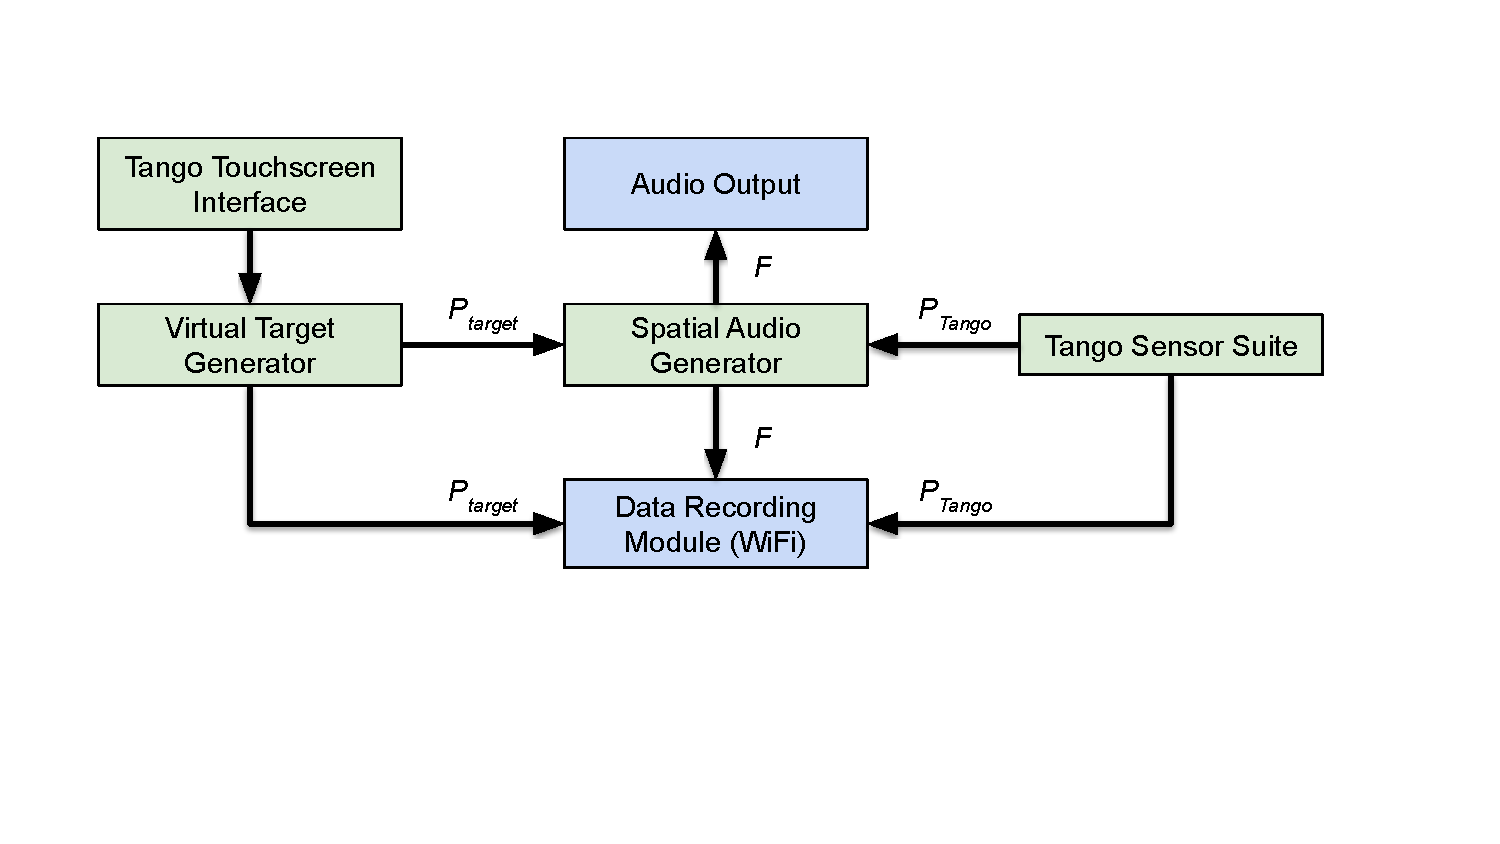
\includegraphics[clip=true, trim=0 120 80 50, width=\columnwidth]{figures/pipeline.pdf}
  \caption{A diagram of the individual system components and their communication pipelines. $F$ indicates a feedback signal and $P$ a pose signal~\citep{lock2019bone}.}\label{fig:pipeline}
\end{figure}

\subsection{Participant Characterisation}\label{sec:participant_characterisation}

A preliminary set of experiments were conducted to characterise the participants' hearing characteristics.
The measured characteristics were each participant's audio localisation ability on the lateral plane, as well as the participants' ability to discriminate between tones with different frequencies. 
These results will be used to provide context to the following target search experiment and provide additional insight on any possible biases or limitations. 

\subsubsection{Sound Localisation} \label{sec:sound_localisation}

In this experiment, we evaluated a participant's ability to determine the lateral direction a sound is coming from.
To do this, we played a continuous \SI{512}{\hertz} sinusoidal tone to the participant through the headphones and applied an HRTF to spatialise and place its source to the participant's left or right.
The participant then had to select the direction the sound came from.
The longer the experiment lasts and the more correct guesses the participant makes, the closer the source moves to the centre-front of the participant, making it increasingly harder to localise. 

For this progressive increase in difficulty, a ``2-up, 1-down'' step process is used~\citep{wetherill1965sequential,levitt1971transformed}, meaning that for every two correct answers, the distance to the centre halves.
Conversely, the task becomes easier for each incorrect answer by doubling the sound source's distance from the centre.
We also use two different step sequences, one starting at a large angular distance (\SI{45}{\degree}) from the user and the other at the minimum distance (approximately \SI{1}{\degree}), giving an `easy' and a `hard' progression respectively.
The terminating condition for the experiment is when the two sequences converge to within two intervals of one another for three consecutive guesses.
For example, the experiment will terminate when one sequence is set to \SI{11.25}{\degree} and the other is between \SI{2.8}{\degree} or \SI{45}{\degree} for three consecutive guesses.
This gives a distance band where the participant is capable of localising the sound source.
Each participant performed this experiment three times. 

\subsubsection{Pitch Discrimination}\label{sec:pitch_discrimination}

Here we determined a participant's ability to differentiate the pitches of two different tones, i.e.\ how well they can tell if a tone is high or low pitched.
We played two tones to the participants, in succession, with the second tone being higher or lower-pitched than the first.
The participants were then asked to select which tone was higher or lower.

The first tone is randomly generated, while the second tone is generated by adding or subtracting some value from the first one.
The tone difference depends on how well the participant can tell the tones apart.
Like the sound localisation experiment, a ``2-up, 1-down'' step process is used: for every two consecutive correct answers, the pitch difference between the tones is halved, while it is doubled for every incorrect answer.
Two-step sequences are again used here, one starting with a large pitch difference ($f_h=2^9=$ \SI{512}{\hertz}) between the tones and the other with a small difference ($f_l=2^1=$ \SI{2}{\hertz}).
The termination condition is when the two-step sequences are within one octave of each other (i.e.\ $\log_2\frac{f_h}{f_l}=2$) for three consecutive answers.
For example, the experiment will terminate when one sequence is set to \SI{64}{\hertz} and the other is between \SI{32}{\hertz} or \SI{128}{\hertz} for three consecutive guesses.
Pitch differences are measured in semitones, which can be obtained with

\begin{equation}
\label{eq:semitone-difference}
  \Delta f = 12\log_2\frac{f_0}{f_1}, 
\end{equation}

\noindent where $f_0$ and $f_1$ are the frequencies of the first and second tone respectively.
Each participant performed this experiment twice. 

\subsection{Target Search}\label{sec:target_search}

To test the interface's effectiveness at guiding the user in a pointing task, a set of experiments were conducted to capture the difference between the targets' actual direction and the directions the participants' perceived them to be.

The participants were given a Tango device running an app that implements the experimental setup in~\Cref{fig:pipeline}. The app generates a set of virtual targets and presents them to each participants through the audio interface, one at a time. 
The targets are generated at a constant distance from the participant and their pan and elevation angles are uniformly generated across the four quadrants of the pan-elevation plane to avoid clustering.
Each target's angular position is adjusted and communicated in real-time as the participant points the device around. 
When the participants were confident that the device was on-target, i.e.~hearing the audio front-on at \SI{512}{\hertz}, they tapped the screen, marking the location and generating the next target.
The targets' positions are all set relative to the device's coordinate system, which is tracked using the Tango hardware and localisation API.\
A total of 28 targets were generated per participant. 

As part of this experiment, we wanted to see how changing the gradient of the pitch function, visualised in~\Cref{fig:pitch-gain}, affected target acquisition performance, e.g.\ does a steeper pitch gain function as a function of the elevation angle improve accuracy or decrease the search time?
Pitch limits of one, two and three octaves above and below the neutral tone were then set for the so-called \textit{lo}, \textit{med} and \textit{hi} pitch gradient settings, respectively.

We use two different metrics to compare the three different pitch gradient settings: acquisition accuracy and search time.
The accuracy is given as the difference between the Tango's orientation at the time the participant confirmed they were on target, and the target's actual orientation.
We separate the results of the tilt and pan dimensions in order to see how the different pitch gradients affect a participant's pointing accuracy. 

We also compare the performance of the three pitch gradient settings in terms of the time it takes each participant to find a target.
However, since each participant was presented with a different, randomly generated set of targets, a direct time comparison is not possible.
Instead, we use Fitts's Law~\citep{fitts1954information}, modified by MacKenzie for uncertain target sizes and noisy data~\citep{mackenzie1992fitts}, which states that there is a relation between the time it takes to find a target and its index of difficulty (the ratio between the distance to the target and its width).
It also provides a so-called `index of performance' that we can use as a metric to compare the results between the three configurations. 

Here we briefly summarise the equations and quantities involved in our metric.
Fitts's Law is given by  

\begin{equation}
  \label{eq:fitts-base}
  t = a + b~ID,
\end{equation}

\noindent
where $t$ is the time it takes to find a target, $a$ and $b$ are constants determined through regression and $ID$ is a description of the difficulty of the target, given as logarithmic function of the ratio between the distance to the target and the target's width.
In our case, the targets have no width, since they are points in space, and we therefore use MacKenzie's modified form for $ID$, given by

\begin{equation}
  \label{eq:fitts-id}
  ID = \log_2\left(\frac{\theta}{w_e} + 1\right).
\end{equation}

\noindent
Here $\theta$ is the angular distance between subsequent target centres and $w_e$ is the targets' effective angular width~\citep{welford1968fundamentals}, given by

\begin{equation}
  \label{eq:fitts-we}
  w_e = \sqrt{2\pi e}~\sigma = 4.133~\sigma,
\end{equation}

\noindent
where $\sigma$ is the standard deviation of the error data, taken as the angle between the participant's target selection and target's actual angular position.
Fitts's index of performance, $IP$, can then be calculated using 

\begin{equation}
  \label{eq:fitts-performance}
  IP = \frac{ID}{t}.
\end{equation}

% \noindent
% where $IP = \frac{1}{t}$ when $\sigma=0$.% When sigma=0, then ID=log2(0/we + 1) = log2(1) = 0

\subsection{Procedure}

Two groups of participants were recruited for the experiments on a volunteer basis. 
Group~\textit{G1} consisted of 42 young adults with normal eyesight who were blindfolded for the experiments, and group \textit{G2} contained 8 people with severe visual impairments (18--55 years old; 36 female, 14 male). 
None of the participants had any hearing or other disabilities that could have influenced their performance in the experiments.
Each participant performed three sets of experiments each, with the two characterisation experiments in \Cref{sec:participant_characterisation} preceding the final target-search experiment in \Cref{sec:target_search}. 
Both groups were given some time before the target-search experiment to familiarise themselves with the system, the audio signal's behaviour and the \SI{512}{\hertz} on-level tone. 
Furthermore, to minimise any potential speed/accuracy biases, we asked the participants to focus on finding the targets without worrying about the time it took to complete the task. 

\section{Results}\label{sec:results}

\subsection{Characterisation of Sound Localisation}

\Cref{fig:sound-localisation} shows the results captured from the sound localisation experiment where the participants had to select the direction (left or right) that the tone was being played from. 
%
It can be seen that the vast majority of guesses for both groups were correct.
For Group~\textit{G1}, most of the errors were made at the minimum distance from the centre, i.e.\ the most difficult to guess correctly, which is the expected behaviour.
This indicates that the participants in \textit{G1} consistently progressed through the distance intervals and we can therefore conclude they had little difficulty determining sound direction.

\begin{figure}
  \centering
  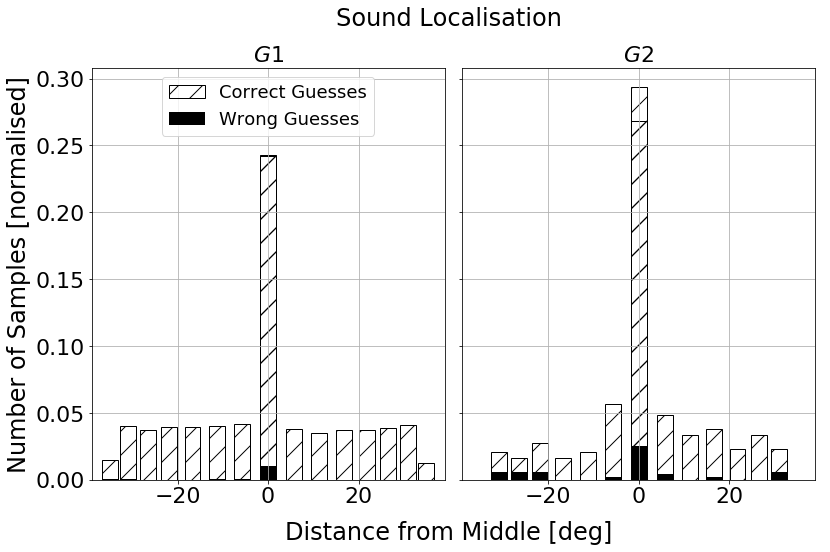
\includegraphics[width=1.0\textwidth]{figures/sound_localisation.png}
  \caption{Histograms of the participants' guesses of the tone locations that show the correct and incorrect guesses for each bin. }\label{fig:sound-localisation}
\end{figure}

Group~\textit{G2} also displays a concentration of erroneous guesses in the central interval.
However, it also shows more errors in other distance intervals and a more even progression towards the centre.
This could indicate that, instead of terminating the experiment as described in \Cref{sec:sound_localisation}, there was more switching back and forth between the three central intervals. 

These results show that both participant groups are capable of determining a sound source's location with a reasonable level of consistency and accuracy.
These results are in line previous literature, confirming that humans are very adept at localising a sound source, particularly in the pan dimension. 

\subsection{Characterisation of Pitch Discrimination}

The results of the pitch discrimination experiment are shown in \Cref{fig:pitch-discrimination}, where bar plots are used to show the proportion of correct to incorrect guesses of which tone was higher pitched for different tone difference intervals. 
For Group~\textit{G1}, we see that their guesses are normally spread around the 0 semitone-difference interval and, as expected, the highest proportion of incorrect guesses occurs in the $[-0.25, 0.25]$ semitone-difference interval. 
The guesses from Group~\textit{G2} are more concentrated around the centre and the majority of incorrect guesses also occurs in the $[-0.25, 0.25]$ semitone-difference interval.

Assuming these differences are normally distributed, we fit a cumulative distribution function (CDF) over each participant's set of results for their correct guesses.
We then used each CDF's parameters to determine a frequency cut-off threshold, where the participant could not longer reliably tell tones apart, which is set to contain 75\% of each participant's correct guesses.
The median of these threshold values can then be used to estimate the frequency difference at which the entire participant population can no longer tell the difference between two tones. 
It can also be used to improve the interface's frequency profile and performance. 
\Cref{fig:pitch-thresholds} shows the threshold distribution, along with the median value, which was found to be approximately 0.4 semitones for each group. 
\Cref{fig:pitch-thresholds-hist} contains histograms of the cut-off frequency thresholds for each setting, which show that the settings can be grouped together.
%The median is used for each grouping given the skewed plot and

\begin{figure}
  \centering
  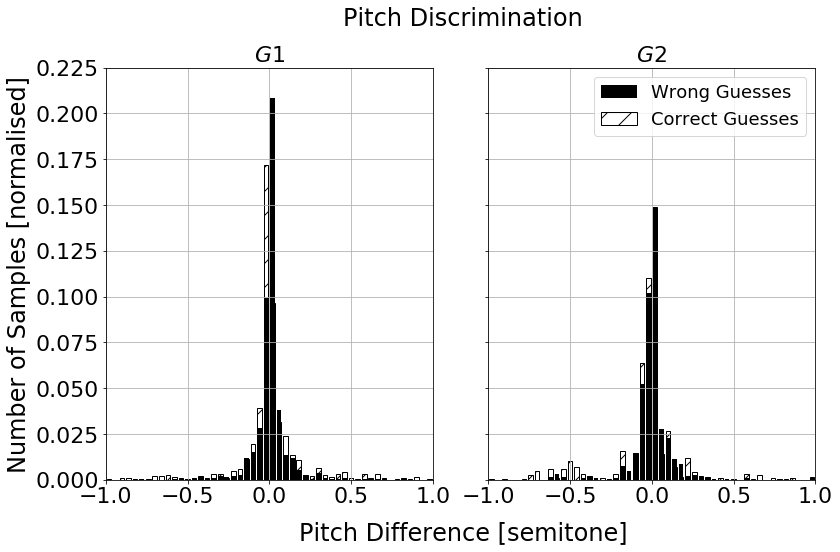
\includegraphics[width=1.0\textwidth]{figures/pitch_discrimination.png}
  \caption{Histograms of the participants' guesses of which tone was higher pitched that show the correct and incorrect guesses for each bin. }\label{fig:pitch-discrimination}
\end{figure}

\begin{figure}
  \centering
  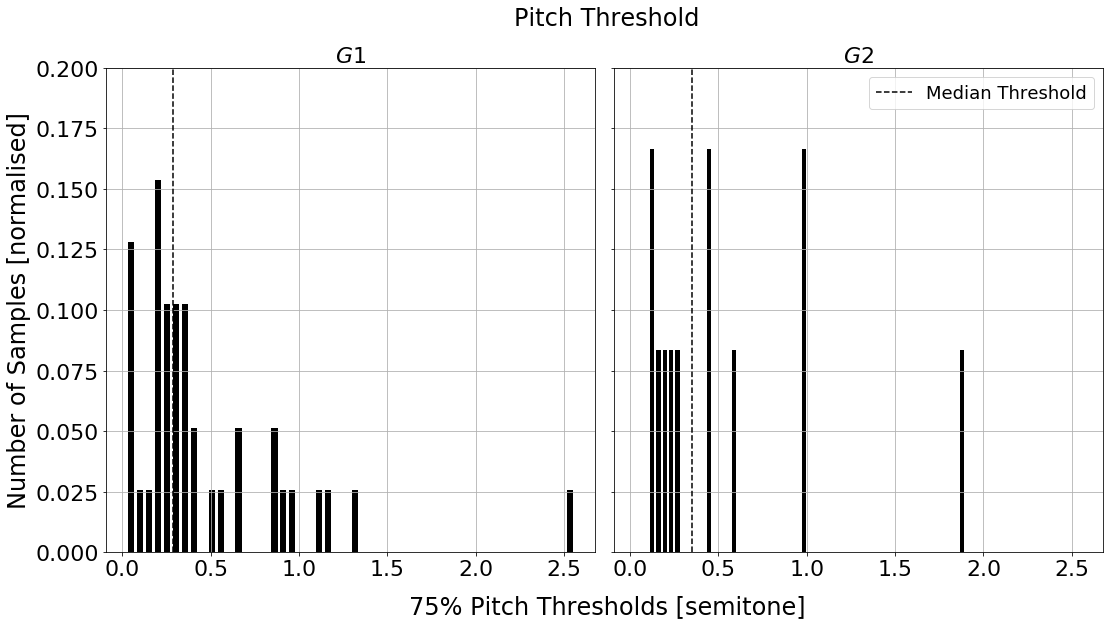
\includegraphics[width=1.0\textwidth]{figures/pitch_thresholds.png}
  \caption{Distributions of the median cut-off frequency thresholds along with the median 75\% cut-off thresholds. }\label{fig:pitch-thresholds}
\end{figure}

\begin{figure}
  \centering
  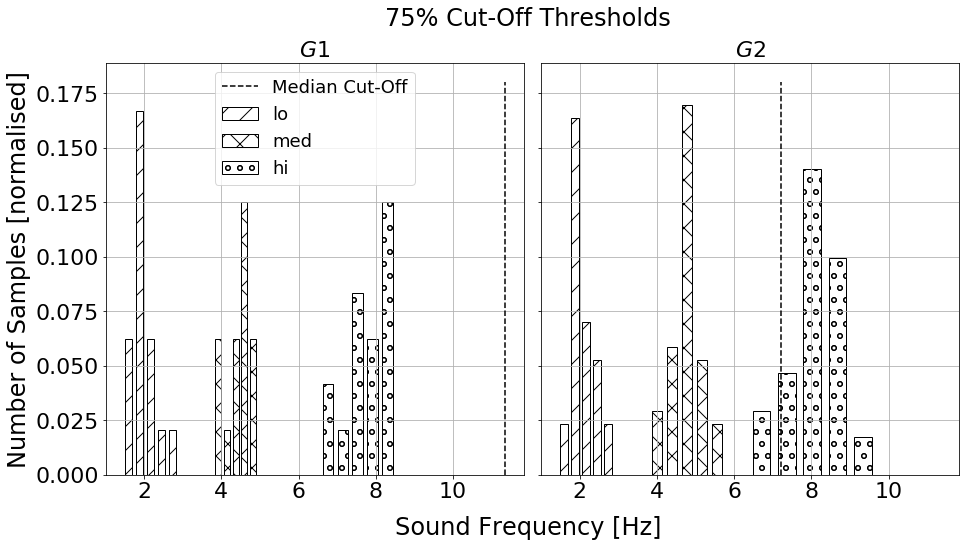
\includegraphics[width=1.0\textwidth]{figures/pitch_thresholds_limits.png}
  \caption{Histogram distributions of the participants' 75\% cut-off thresholds. }\label{fig:pitch-thresholds-hist}
\end{figure}

\subsection{Target Search}

The results from the target search experiment shown on the 2D histograms in \Cref{fig:target-errors}, where the angular errors in the pan and elevation dimensions are plotted against each other. 
A set of box-plots of the angle errors are also given in \Cref{fig:target-boxplot-error} for each audio setting.
The results are summarised in \Cref{tab:target-results}.

\begin{figure}
  \centering
  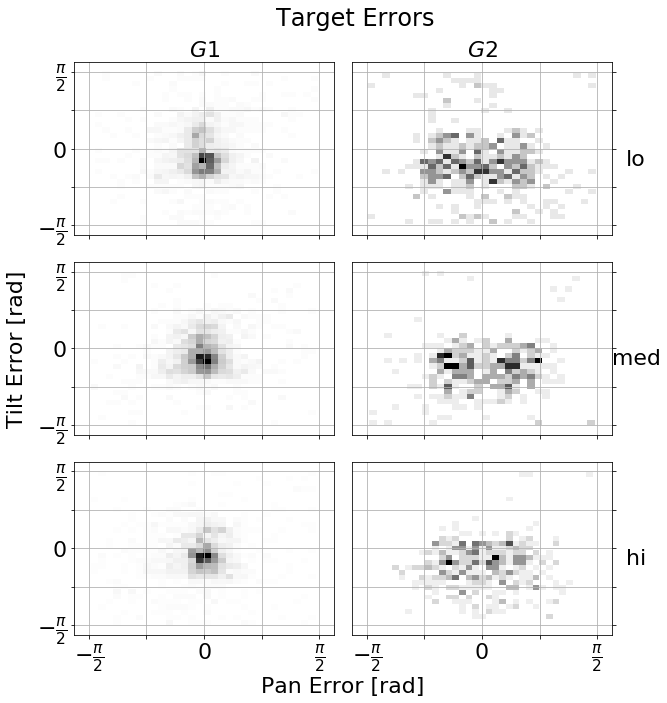
\includegraphics[width=1.0\textwidth]{figures/target_errors.png}
  \caption{Distributions of the angular errors in the pan and elevation dimensions for the 3 different pitch gradient settings. }\label{fig:target-errors}
\end{figure}

\begin{figure}[t]
  \centering
  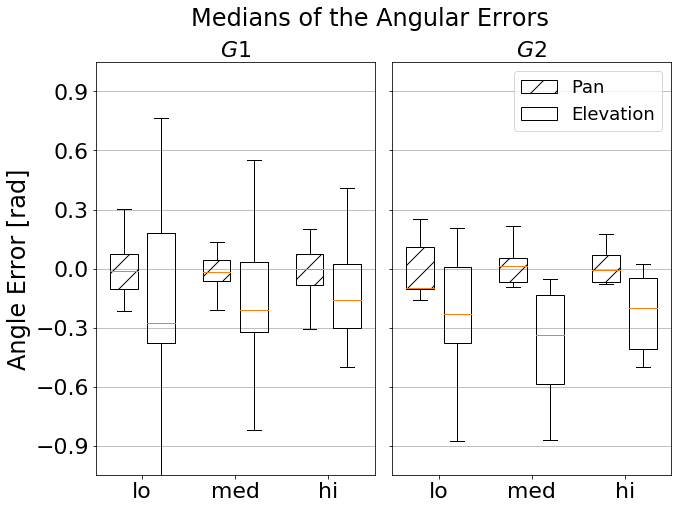
\includegraphics[width=1.0\textwidth]{figures/boxplot_target_search_median_error.png}
  \caption{Box-plots of the median pan and elevation errors for each audio setting. }\label{fig:target-boxplot-error}
\end{figure}

\begin{table}
  \centering
  \caption{The average target acquisition error in the pan and elevation dimensions for each participant group. }\label{tab:target-results}
  \begin{tabular}{p{0.5cm}p{1.5cm}p{1.5cm}p{3.0cm}p{3.0cm}p{3.0cm}}
    \toprule
    &           & Setting      & Mean Angle Error [rad] & Mean Absolute Angle Error [rad] &  Pearson Correlation \\ \midrule
    \multirow{6}{*}{\textit{G1}}
    &           & \textit{lo}  & $-0.02\pm0.37$ & $0.25\pm0.27$ & $0.75,~p < 0.001$ \\
    & Pan       & \textit{med} & $-0.01\pm0.37$ & $0.26\pm0.27$ & $0.77,~p < 0.001$ \\
    &           & \textit{hi}  & $-0.03\pm0.39$ & $0.26\pm0.29$ & $0.72,~p < 0.001$ \\ \cline{2-6}
    &           & \textit{lo}  & $-0.12\pm0.51$ & $0.42\pm0.31$ & $0.36,~p < 0.001$ \\
    & Elevation & \textit{med} & $-0.11\pm0.41$ & $0.44\pm0.24$ & $0.49,~p < 0.001$ \\
    &           & \textit{hi}  & $-0.15\pm0.44$ & $0.36\pm0.29$ & $0.48,~p < 0.001$ \\ \midrule
    \multirow{6}{*}{\textit{G2}}
    &           & \textit{lo}  & $-0.01\pm0.37$ & $0.48\pm0.31$ & $0.10,~p = 0.03$  \\
    & Pan       & \textit{med} & $ 0.04\pm0.53$ & $0.45\pm0.27$ & $0.13,~p = 0.01$  \\
    &           & \textit{hi}  & $ 0.03\pm0.48$ & $0.36\pm0.22$ & $0.21,~p < 0.001$ \\\cline{2-6}
    &           & \textit{lo}  & $-0.30\pm0.59$ & $0.49\pm0.39$ & $0.03,~p = 0.48$  \\
    & Elevation & \textit{med} & $-0.42\pm0.45$ & $0.42\pm0.33$ & $0.31,~p < 0.001$ \\
    &           & \textit{hi}  & $-0.37\pm0.43$ & $0.36\pm0.32$ & $0.40,~p < 0.001$ \\ 
    \bottomrule
  \end{tabular}
\end{table}

The Shapiro-Wilkes test for normality reveals that none of these distributions are normally spread. Therefore, the Pearson test is used to investigate the correlation between the actual target location and participants' pointing location.
These results are included in \Cref{tab:target-results}.
The Pearson correlation scores for Group~\text{G1} indicate a moderate to strong positive correlation between the target and the selected locations ($r_{pan} \in [0.72, 0.77],~p < 0.001;~r_{elevation} \in [0.36, 0.49],~p < 0.001$), showing that both the pan and elevation cues in general worked as expected.
However, the correlation scores for Group~\textit{G2} are significantly weaker, with a pan angle correlation $r_{pan} \in [0.1, 0.21],~p < 0.03$.
With the exception of the \textit{lo} setting ($p_{lo} = 0.48$), the elevation correlation is generally stronger, with $r_{elevation} \in [0.31, 0.40],~p < 0.001$.

The repeated-measures procedure that was used for these experiments requires the data for each participant to be grouped together for each setting.
The medians of these data groupings are then used as individual samples that represent an individual participant's performance for each setting.
\Cref{fig:target-boxplot-error} shows these median data collected from each participant as a set of box-plots, while \Cref{fig:target-boxplot-absolute-errors} shows the collection of absolute errors.

\begin{figure}[t]
  \centering
  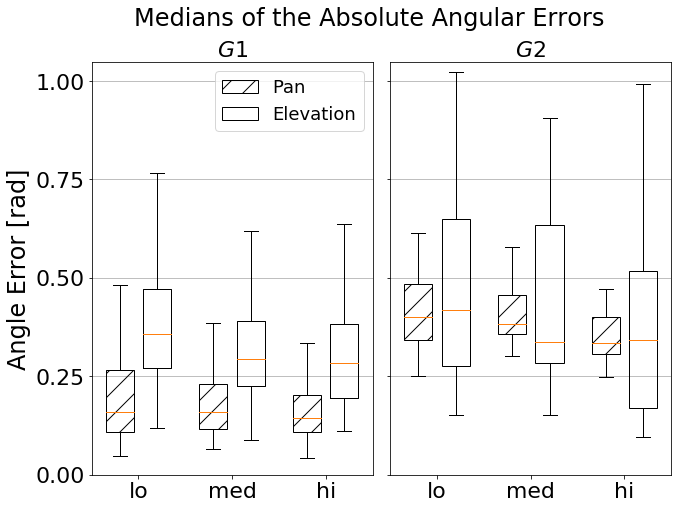
\includegraphics[width=1.0\textwidth]{figures/boxplot_target_search_absolute_median_error.png}
  \caption{Distributions of the absolute angular errors in the pan and elevation dimensions for the 3 different pitch gradient settings. }\label{fig:target-boxplot-absolute-errors}
\end{figure}

The box-plots in \Cref{fig:target-boxplot-error} show that the error in the pan dimension is approximately centred around \SI{0}{\radian} for both groups, with some divergence between the groups for the different settings.
However, using the Friedman test for repeated measures on the medians of absolute errors, these divergences are found to be not significant ($p_{G1} = 0.17,~p_{G2} = 0.09$), showing that spatial perception and accuracy are not affected by changes in the tone's pitch.
This is further demonstrated in the box-plots in \Cref{fig:target-boxplot-absolute-errors}, which demonstrates relatively consistent error levels in the pan dimension for both groups and across all three settings. 

Regarding the errors in the elevation dimension in \Cref{fig:target-boxplot-error}, we observe in Group~\textit{G1} a narrowing distribution between the \textit{lo}, \textit{med} and \textit{hi} settings, respectively, and a median gradually approaching \SI{0}{\radian}.
A similar trent is observed for Group~\textit{G2}, but the improvement across the settings is more subtle and not as linear as for Group~\textit{G1}.
\Cref{fig:target-boxplot-absolute-errors} shows a clearer improvement, i.e.\ approaching \SI{0}{\radian}, for the elevation data between the three settings in both groups, with the \textit{hi} setting producing the smallest error in both cases.
Further analysis of the medians of the absolute elevation error with the Friedman test reveals that the results for the different settings are significantly different from each other only for Group~\textit{G1} ($p_{G1} = 0.002,~p_{G2} = 0.32$).

A post-hoc analysis using the Wilcoxon signed rank test, with a Holm-Bonferroni correction applied to the commonly used 0.05 threshold, was used to investigate the setting relationships more closely. 
This analysis reveals that there is a significant difference between the errors generated by the \textit{lo} and \textit{med} settings, as well as the \textit{lo} and \textit{hi} settings, for Group~\textit{G1} ($p_{lo-med} = 0.003,~p_{lo-hi} < 0.001$), showing that the \textit{lo} setting clearly produces the highest error, while it is not clear which one of the \textit{med} and \textit{hi} settings is better for Group~\textit{G1}. 
Based on the current data, it is impossible to conclude which setting produces the smallest angular error for Group~\textit{G2}, but this may be caused by the relatively small sample size for each setting. 
%while Group~\textit{G2} has 2 significantly different levels of performance between the \textit{lo} and \textit{med} settings, as well as for the \textit{med} and \textit{hi} settings ($p_{lo-med} = 0.011, p_{med-hi} = 0.001$).
We also noted that there is a significant negative error bias in the elevation for all the settings and groups, possibly caused by a cognitive constraint introduced by the floor, below which the participants believed the targets could not appear.
Since this bias seems to be constant, it could be easily addressed in a future version of the audio interface by adjusting its frequency parameters to shift the bias upwards by a constant offset. 

Comparing the distributions for each setting between the two groups with the Kruskal-Wallis test for non-parametric data, we see that the differences between the distributions for all three settings are not significantly different, for both groups and both pan and elevation (the $p$-values are summarised in \Cref{tab:inter-group-results}).
This results confirm that the performance of the blindfolded participants and those with severe sight impairments are statistically similar, and that groups from a different population can reasonably be expected to produce similar errors, under similar experimental conditions. 
Consequently, we can conclude that the \textit{hi} setting, which generates the significantly smallest elevation error, is the best audio pitch level to guide a user in a pointing task, and that the pan error is completely independent of such setting choice. 

\begin{table}
  \centering
  \caption{A summary of the $p$-values comparing the distributions of the different settings' error data for each group in both the pan and elevation dimensions. }\label{tab:inter-group-results}
  \begin{tabular}{lll}
    \toprule
                   & Pan      & Elevation \\ \midrule
      \textit{lo}  & $p=0.18$ & $p=0.90$  \\
      \textit{med} & $p=0.86$ & $p=0.34$  \\
      \textit{hi}  & $p=0.28$ & $p=0.38$  \\
    \bottomrule
  \end{tabular}
\end{table}

\subsection{Time-to-Target}

To investigate if the interface generates a Fitts-like response from the participants, we plot the time to find the target as a function of the targets' indices of difficulty, as defined by \Cref{eq:fitts-base}.
The data is binned in intervals of the effective target width~($w_e$), given by \Cref{eq:fitts-we}, and are plotted for each pitch gradient setting. 
A logarithmic line is fitted through the bins' median values by regression and all the results are presented in \Cref{fig:fitts-results}.

\begin{figure}
  \centering
  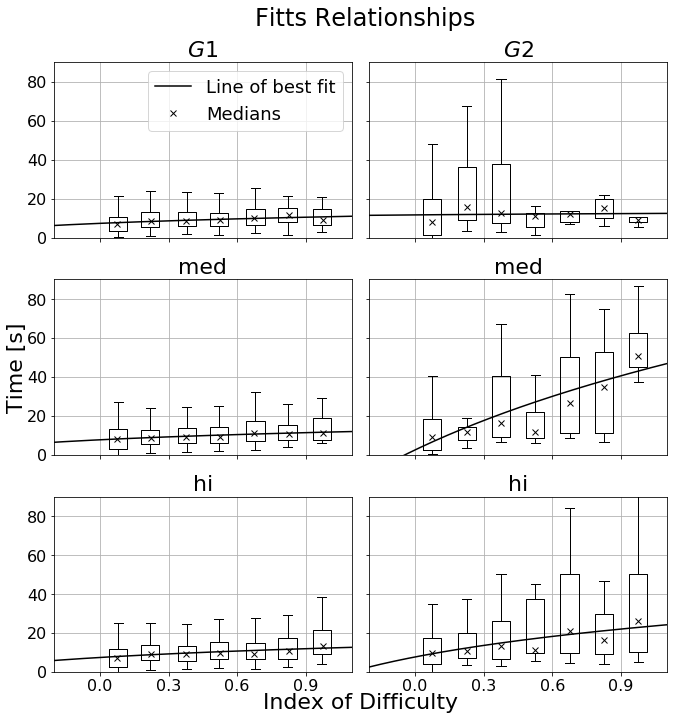
\includegraphics[width=1.0\textwidth]{figures/fitts_fit.png}
  \caption{Plots showing the Fitts relationship between the time it took the participants to find a target and the target's index of difficulty. }\label{fig:fitts-results}
\end{figure}

For Group~\textit{G1}, a Fitts relationship can be observed and the logarithmic line of best fit closely approximates the median values of the binned data for all three settings. 
This is confirmed by strong Pearson correlation scores for each setting ($r_{lo} = 0.76,~p_{lo} = 0.045;~r_{med} = 0.96,~p_{med}<0.001;~r_{hi} = 0.86,~p_{hi} = 0.013$).
Regarding Group~\textit{G2}¸ we observe larger spreads for each binned data plot, indicating less consistency in the time-to-target results for participants with severe sight impairments.
This could be due to each participant's result being taken as a single datum and to the smaller population size in Group~\textit{G2}.
Nevertheless, the \textit{med} and \textit{hi} settings exhibit strong Pearson correlation scores ($r_{med} = 0.88,~p_{med} = 0.008;~r_{hi} = 0.84,~p_{med} = 0.017$), while the results for the \textit{lo} setting does not produce a statistically significant correlation ($r_{lo} = 0.08,~p_{lo} = 0.85$).

\begin{figure}[t]
  \centering
  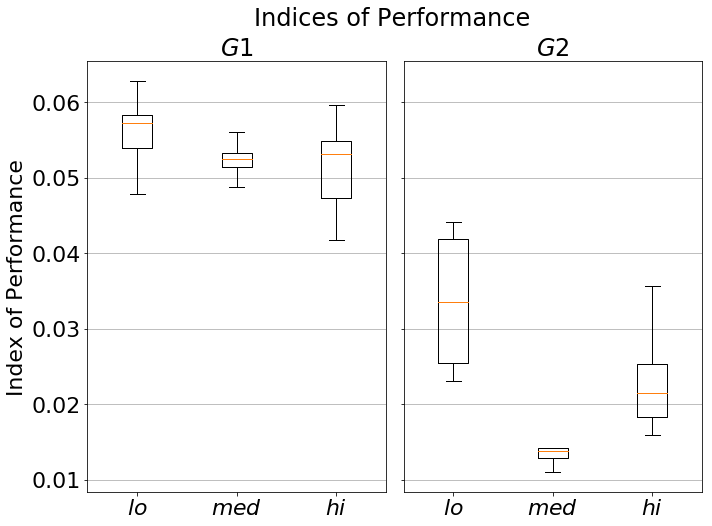
\includegraphics[width=1.0\textwidth]{figures/fitts_ips.png}
  \caption{Plots showing the Fitts relationship between the time it took the participants to find a target and the target's index of difficulty. }\label{fig:fitts-ips}
\end{figure}

These results allows us to calculate and plot in \Cref{fig:fitts-ips} an index of performance, as given by \Cref{eq:fitts-performance}, for each audio setting.
The results are summarised in \Cref{tab:fitts-results}.
For Group~\textit{G1}, there is a fairly consistent level of performance between the three settings, with \textit{lo} producing the highest indices of performance overall (i.e.\ the participants found the targets with the smallest error and in the least amount of time).
This is supported by the results from the Friedman test, showing that there is a significant difference in performance between the settings ($p < 0.001$), as well as post-hoc Wilcoxon tests with Holm-Bonferroni corrections, which show that the \textit{lo} setting is significantly different to the \textit{med} and \textit{hi} settings ($p_{lo-med} < 0.001,~p_{lo-hi} < 0.001$). The \textit{med} and \textit{hi}, instead, are not significantly different from each other ($p_{med-hi} = 0.85$).
The results for Group~\textit{G2} show generally lower and inconsistent indices of performance for each setting, which is expected given the increased times to target observed in \Cref{fig:fitts-results}.
Again, from the Friedman test ($p < 0.001$), the \textit{lo} setting produces the highest performance by a large margin, compared to the \textit{med} setting, with the Wilcoxon test and Holm-Bonferronni corrections ($p_{lo-med}=0.01$), followed by the \textit{hi} and \textit{med} settings' results, respectively.
This seems to indicate that, for both groups, the \textit{lo} setting produces the highest level of performance, followed by the \textit{hi} setting.

\begin{table}
  \centering
  \caption{The average target acquisition error in the pan and elevation dimensions for each participant group. }\label{tab:fitts-results}
  \begin{tabular}{p{0.5cm}p{1.5cm}p{2.5cm}}
    \toprule
    & Setting      & Mean Index of Performance \\ \midrule
    & \textit{lo}  & $0.056\pm0.005$ \\
    \textit{G1} & \textit{med} & $0.053\pm0.008$ \\
		& \textit{hi}  & $0.051\pm0.007$ \\ \cline{2-3}
    & \textit{lo}  & $0.034\pm0.009$ \\
    \textit{G2} & \textit{med} & $0.014\pm0.002$ \\
    & \textit{hi}  & $0.022\pm0.006$ \\
    \bottomrule
  \end{tabular}
\end{table}

\Cref{fig:fitts-ips} shows a significant difference between the IPs for each group's respective settings, with \textit{G2} producing significantly lower indices of performance.
This is further supported by the Kruskal-Wallis test, revealing that each setting's distribution is indeed significantly different from its counterpart in the other group ($p_{lo} < 0.001,~p_{med} < 0.001,~p_{hi} < 0.001$).
The significant difference between the blindfolded group and the group of participants with visual impairments seems to indicate that the latter require significantly more time to find the target. 
However, it is unclear whether this is a systematic cause or a difference in search strategy between the two groups, e.g.\ \textit{G2} preferring, on average, a slower and more methodical approach.

\subsection{Discussion}

The results for the accuracy and time performance with the proposed audio interface shows an interesting contrast.
That is, the \textit{hi} pitch setting produces the lowest target acquisition error, followed by the \textit{med} and \textit{lo} settings, respectively. 
However, this trend is almost wholly reversed in the time-to-target results from the Fitts's model, where the \textit{lo} setting gives the highest level of performance, followed by the \textit{hi} and \textit{med} settings respectively. 
Since the Fitts's model takes the angular error into account, one might reasonably expect that the results for both experiments follow a similar trend. 
However, the Fitts's model does not account for different stimuli.
We therefore hypothesise that the reason for this divergence in performance is due to the increased resolution of the \textit{hi} setting, which allows for finer adjustments of the device's orientation, getting it closer to the correct target, but at the cost of a higher average time-to-target. 
This seems to indicate a speed/accuracy trade-off in finding the targets.
With the Fitts's model discussed here, we can modify the interface to prioritise different metrics and produce the correct output. 

Regarding target acquisition, the progressive improvement from the \textit{lo}, \textit{med} and \textit{hi} settings (see \Cref{tab:target-results}) seems to indicate that simply increasing the pitch gradient leads to better target-pointing performance.
However, \Cref{fig:pitch-thresholds-hist} shows that the frequency difference between the ``on-target'' tone and the selected one with the \textit{hi} setting approaches the cut-off frequency of Group~\textit{G1}, indicating an inflection point where increasing the gradient reduces the final performance. 
Indeed, the participants from Group~\textit{G2} seem to go beyond this threshold and reach a saturation point where they can no longer reliably distinguish different tones.  

\section{Conclusion}\label{sec:conclusion}

In this paper we investigated the use of spatialised audio interface with varying pitch to guide a visually impaired user in a target pointing task.
We found that the blindfolded participants and those with severe sight impairments performed similarly in localising sound sources and differentiating between tones. 
We also found that both groups were able to find a randomly distributed set of virtual targets with similar levels of accuracy.
However, the blindfolded group outperformed the one with severe sight impairments in terms of time-to-target. 
We further tested different pitch settings and found that the user performance in the pan dimension, based on spatialised cues, is independent of such settings.
Moreover, we noticed a speed/accuracy trade-off between the settings, where a higher pitch setting produces a smaller angular error, but at the cost of reducing the time performance (i.e.\ more time to reach the target). 
These results, together with an analysis done with Fitts's Law confirms its applicability to this type of audio interface, provide a useful baseline to improve and refine the latter in future applications, prioritising speed or accuracy to produce the desired output.

This work identified a number of uncertainties that can be the focus of future work.
These include questions such as what caused the observed difference in time performance between the groups and whether the constant negative bias observed in \Cref{fig:target-boxplot-error} is indeed caused by a cognitive bias within the participants' minds, or whether there is a more complex underlying reason for the behaviour.
Furthermore, casual post-experiment conversations with the participants revealed that some felt that one setting was easier to understand than the others and it can therefore be beneficial to investigate the possibility of adding an auto-adaptation component to the audio signal.
For example, the pitch gradient can be automatically adjusted over time by the device to provide a better match between the human and computer and increase overall target-finding performance.
Indeed, the work by~\cite{gallina2015progressive} may serve as a good guideline for such a system.
Additional feedback modes may also be added to allow for clearer guidance experience for the user, e.g.\ vibration signals to inform them when they point to the target or adjusting the volume to expand the system to three dimensions.
With this kind of audio interface now better understood, it is ready to be implemented into a fully packaged guidance system for people with visual impairments.

\section*{Acknowledgements}

This project is partly funded and supported by the Google Winter Award (2016).

\bibliographystyle{apacite}
\bibliography{bib}

\end{document}
